% !TeX TXS-program:bibliography = txs:///bibtex
%oli8: this line allows me to use plain BibTex without reconfiguring
%my own settings. 

%BEGIN_FOLD  AAAI-preamble
\def\year{2021}\relax
% File: formatting-instruction.tex
\documentclass[letterpaper]{article} % DO NOT CHANGE THIS
\usepackage{aaai21} % DO NOT CHANGE THIS
\usepackage{times} % DO NOT CHANGE THIS
\usepackage{helvet} % DO NOT CHANGE THIS
\usepackage{courier} % DO NOT CHANGE THIS
\usepackage[hyphens]{url} % DO NOT CHANGE THIS
\usepackage{graphicx} % DO NOT CHANGE THIS
\urlstyle{rm} % DO NOT CHANGE THIS
\def\UrlFont{\rm} % DO NOT CHANGE THIS
\usepackage{graphicx} % DO NOT CHANGE THIS
\usepackage{natbib} % DO NOT CHANGE THIS OR ADD OPTIONS
\usepackage{caption} % DO NOT CHANGE THIS OR ADD OPTIONS
\frenchspacing % DO NOT CHANGE THIS
\setlength{\pdfpagewidth}{8.5in} % DO NOT CHANGE THIS
\setlength{\pdfpageheight}{11in} % DO NOT CHANGE THIS
%
% PDF Info Is REQUIRED.
% For /Author, add all authors within the parentheses,
% separated by commas. No accents or commands.
% For /Title, add Title in Mixed Case.
% No accents or commands. Retain the parentheses.
\pdfinfo{
	/Title (Probabilisti Dependency Graphs)
	/Author (Oliver Richardson, Joseph Halpern)
	/TemplateVersion (2021.1)
}
%oli21: enabling subsection numbers (0: no numbers, 1: section, 2: subsection)
\setcounter{secnumdepth}{2} 
%END_FOLD   AAAI-preamble

%BEGIN_FOLD Tikz Stylings.
\usepackage{tikz}
\usetikzlibrary{positioning,fit,calc, decorations, arrows, shapes, shapes.geometric}
\usetikzlibrary{backgrounds}
\usetikzlibrary{cd}

\pgfdeclaredecoration{arrows}{draw}{
	\state{draw}[width=\pgfdecoratedinputsegmentlength]{%
		\path [every arrow subpath/.try] \pgfextra{%
			\pgfpathmoveto{\pgfpointdecoratedinputsegmentfirst}%
			\pgfpathlineto{\pgfpointdecoratedinputsegmentlast}%
		};
}}
%%%%%%%%%%%%
\tikzset{AmpRep/.style={ampersand replacement=\&}}
\tikzset{center base/.style={baseline={([yshift=-.8ex]current bounding box.center)}}}
\tikzset{is bn/.style={background rectangle/.style={fill=blue!35,opacity=0.3, rounded corners=5},show background rectangle}}

% Node Stylings
\tikzset{dpadded/.style={rounded corners=2, inner sep=0.7em, draw, outer sep=0.3em, fill={black!50}, fill opacity=0.08, text opacity=1}}
\tikzset{dpad0/.style={outer sep=0.05em, inner sep=0.3em, draw=gray!75, rounded corners=4, fill=black!08, fill opacity=1}}
\tikzset{dpad/.style args={#1}{every matrix/.append style={nodes={dpadded, #1}}}}
\tikzset{light pad/.style={outer sep=0.2em, inner sep=0.5em, draw=gray!50}}

\tikzset{arr/.style={draw, ->, thick, shorten <=3pt, shorten >=3pt}}
\tikzset{arr0/.style={draw, ->, thick, shorten <=0pt, shorten >=0pt}}
\tikzset{arr1/.style={draw, ->, thick, shorten <=1pt, shorten >=1pt}}
\tikzset{arr2/.style={draw, ->, thick, shorten <=2pt, shorten >=2pt}}
\tikzset{archain/.style args={#1}{arr, every arrow subpath/.style={draw,arr, #1}, decoration=arrows, decorate}}


\tikzset{fgnode/.style={dpadded,inner sep=0.6em, circle},
	factor/.style={light pad}}	


\newcommand\cmergearr[4]{
	\draw[arr,-] (#1) -- (#4) -- (#2);
	\draw[arr, shorten <=0] (#4) -- (#3);
}
\newcommand\mergearr[3]{
	\coordinate (center-#1#2#3) at (barycentric cs:#1=1,#2=1,#3=1.2);
	\cmergearr{#1}{#2}{#3}{center-#1#2#3}
}
\newcommand\cunmergearr[4]{
	\draw[arr,-, , shorten >=0] (#1) -- (#4);
	\draw[arr, shorten <=0] (#4) -- (#2);
	\draw[arr, shorten <=0] (#4) -- (#3);
}
\newcommand\unmergearr[3]{
	\coordinate (center-#1#2#3) at (barycentric cs:#1=1.2,#2=1,#3=1);
	\cunmergearr{#1}{#2}{#3}{center-#1#2#3}
}


\usetikzlibrary{matrix}
\tikzset{toprule/.style={%
		execute at end cell={%
			\draw [line cap=rect,#1] 
			(\tikzmatrixname-\the\pgfmatrixcurrentrow-\the\pgfmatrixcurrentcolumn.north west) -- (\tikzmatrixname-\the\pgfmatrixcurrentrow-\the\pgfmatrixcurrentcolumn.north east);%
		}
	},
	bottomrule/.style={%
		execute at end cell={%
			\draw [line cap=rect,#1] (\tikzmatrixname-\the\pgfmatrixcurrentrow-\the\pgfmatrixcurrentcolumn.south west) -- (\tikzmatrixname-\the\pgfmatrixcurrentrow-\the\pgfmatrixcurrentcolumn.south east);%
		}
	},
	leftrule/.style={%
		execute at end cell={%
			\draw [line cap=rect,#1] (\tikzmatrixname-\the\pgfmatrixcurrentrow-\the\pgfmatrixcurrentcolumn.north west) -- (\tikzmatrixname-\the\pgfmatrixcurrentrow-\the\pgfmatrixcurrentcolumn.south west);%
		}
	},
	rightrule/.style={%
		execute at end cell={%
			\draw [line cap=rect,#1] (\tikzmatrixname-\the\pgfmatrixcurrentrow-\the\pgfmatrixcurrentcolumn.north east) -- (\tikzmatrixname-\the\pgfmatrixcurrentrow-\the\pgfmatrixcurrentcolumn.south east);%
		}
	},
	table with head/.style={
		matrix of nodes,
		row sep=-\pgflinewidth,
		column sep=-\pgflinewidth,
		nodes={rectangle,minimum width=2.5em, outer sep=0pt},
		row 1/.style={toprule=thick, bottomrule},
	}
}
%oli8: disable tikz externalization for now, dependence on etoolbox
% \usepackage{etoolbox}
% \usetikzlibrary{external}
% \tikzexternalize[prefix=tikz/]  % activate!
% %
% \AtBeginEnvironment{tikzcd}{\tikzexternaldisable} %... except careful of tikzcd...
% \AtEndEnvironment{tikzcd}{\tikzexternalenable}
%END_FOLD

%BEGIN_FOLD: Theorems and Tools

\usepackage{booktabs}       % professional-quality tables
\usepackage{amsfonts}       % blackboard math symbols
\usepackage{nicefrac}       % compact symbols for 1/2, etc.
\usepackage{microtype}      % microtypography
\usepackage{mathtools}		%also loads amsmath
\usepackage{amssymb, bbm}

%oli20: oops, this is vorboten :(
% \usepackage[format=plain,
%             labelfont={sl},
%             textfont={it,small}]{caption}

\usepackage{relsize}
\usepackage{environ} % http://ctan.org/pkg/environ; for capturing body as a parameter for idxmats

\usepackage{color}
%\usepackage{stmaryrd}

\usepackage{amsthm}
\usepackage{thmtools}

\theoremstyle{plain}
\newtheorem{theorem}{Theorem}[section]
\newtheorem{coro}{Corollary}[theorem]
\newtheorem{prop}[theorem]{Proposition}
\newtheorem{lemma}[theorem]{Lemma}
\newtheorem{fact}[theorem]{Fact}
\newtheorem{conj}[theorem]{Conjecture}

\theoremstyle{definition}

% no section numbers for theorems in AAAI style ... 
%joe17: can you reinstate this?
%oli20:done
\declaretheorem[name=Definition,qed=$\square$,numberwithin=section]{defn} %
\declaretheorem[name=Construction,qed=$\square$,sibling=defn]{constr}
\declaretheorem[qed=$\square$]{example}

\theoremstyle{remark}
\newtheorem*{remark}{Remark}

\usepackage{xstring}
\usepackage{enumitem}

\newcommand\numberthis{\addtocounter{equation}{1}\tag{\theequation}}

%oli20: apparently this is not allowed in AAAI style.
%oli21: but it helps me edit so I'm reenabling it until later
%FIXME
\usepackage{hyperref}
\definecolor{deepgreen}{rgb}{0,0.5,0}
\hypersetup{colorlinks=true, linkcolor=deepgreen, urlcolor=magenta, citecolor=deepgreen}
%\hypersetup{colorlinks=true, linkcolor=blue!50!black, urlcolor=magenta, citecolor=deepgreen}

\usepackage[noabbrev,nameinlink,capitalize]{cleveref}
\crefname{example}{Example}{Examples}
\crefname{defn}{Definition}{Definitions}
\crefname{prop}{Proposition}{Propositions}
\crefname{constr}{Construction}{Constructions}
\crefname{conj}{Conjecture}{Conjectures}
\crefname{fact}{Fact}{Facts}
\crefname{coro}{Corolary}{Corolaries}
%\crefname{section}{\S\!}{\S\!}


\usepackage{float}
\usepackage{subcaption}
\captionsetup[subfigure]{subrefformat=simple,labelformat=simple}
\renewcommand\thesubfigure{(\alph{subfigure})}

\newenvironment{old}[1]{\par\noindent{\bf \Cref{#1}.} \em \noindent}{\par\medskip}

\usepackage{xpatch}
\makeatletter
\xpatchcmd{\thmt@restatable}% Edit \thmt@restatable
{\csname #2\@xa\endcsname\ifx\@nx#1\@nx\else[{#1}]\fi}% Replace this code
% {\ifthmt@thisistheone\csname #2\@xa\endcsname\typeout{oiii[#1;#2\@xa;#3;\csname thmt@stored@#3\endcsname]}\ifx\@nx#1\@nx\else[#1]\fi\else\csname #2\@xa\endcsname\fi}% with this code
{\ifthmt@thisistheone\csname #2\@xa\endcsname\ifx\@nx#1\@nx\else[{#1}]\fi
	\else\fi}
{\typeout{oii Success1?}}{\typeout{oiii failure1?}} % execute code for success/failure instances
\xpatchcmd{\thmt@restatable}% Edit \thmt@restatable
{\csname end#2\endcsname}
{\ifthmt@thisistheone\csname end#2\endcsname\else\fi}
{\typeout{oii Success2?}}{\typeout{oiii failure2?}}
\newcommand{\recall}[1]{\medskip\par\noindent{\bf \expandarg\Cref{thmt@@#1}.} \begingroup\em \noindent
	\expandafter\csname#1\endcsname* \endgroup\par\smallskip}
\makeatother
%oli16: The extra space was because there was extra space in the paragraph, not
%because this length was too big. By breaking arrays, everything will be better.
\allowdisplaybreaks
%END_FOLD

\newcommand{\begthm}[3][]{\begin{#2}[{name=#1},restate=#3,label=#3]}
	
	%TODO
	\newcommand{\createversion}[2][{gray}{0.75}]{
		\definecolor{v#2color}#1\relax
		\expandafter\xdef\csname v#2on\endcsname{%
			% \xdef\gamma{\tau}%
			% \expandafter\renewcommand\csname v#2\endcsname{ONN}%
			% \expandafter\xdef{\csname v#2on\endcsname}##{{\color{v##2color} #1}}
		}
		\expandafter\xdef\csname v#2off\endcsname{
			% 	\expandafter\newcommand\csname v #2\endcsname[1]{{\color{v ##2 color} #1}}
		}
	}
	\createversion{test}
	% \vteston

	
%BEGIN_FOLD   %%%% Version knobs %%%%%. 
%oli20: your commenting system is better than the one based on comment package, 
% which is way more problematic than I thought.
% I'm killing it and refactoring all comments to be like yours. I'm not annotating
% everything I'm doing here but the result will be way clearer and less problematic.

\definecolor{vfullcolor}{gray}{0.7}
\newcommand\vfull[1]{{\color{vfullcolor} #1}}
\renewcommand\vfull[1]{} % disable vfull

\definecolor{vleftoverscolor}{gray}{0.85}
\newcommand{\vleftovers}[1]{{\color{vleftoverscolor} #1}} 
\renewcommand{\vleftovers}[1]{} %disable vleftovers

\definecolor{notationcolor}{rgb}{0.9,0.9,.9} 
\newcommand{\notation}[1]{{\color{notationcolor} #1}}
\renewcommand{\notation}[1]{\ignorespaces} % disable notation

\definecolor{contentiouscolor}{rgb}{0.7,0.3,.1} 
\newcommand{\commentout}[1]{\ignorespaces} 

% \newcommand{\contentious}[1]{
% 	\noindent\colorbox{red!10!white}{\parbox{\linewidth-3pt}{\color{red!10!black}#1}}}
% \newcommand{\valpha}[1]{%
% 	% \colorbox{red!10!white}
% 	{\color{red!10!black}{#1}}%
% }
% \newenvironment{\valpha}{\begingroup}
\newcommand{\valpha}[1]{{\color{red!80!black}#1}}
% \renewcommand{\valpha}[1]{\ignorespaces} 
\newcommand{\attn}[1]{{\color{violet!50!cyan}#1}}
%END_FOLD

	
%BEGIN_FOLD definitions
%BEGIN_FOLD %%%%%   general shorthand I use   %%%%%%%%%%%%%%%%%

%\usepackage{stmaryrd}
%\DeclarePairedDelimiter{\ccbr}{\lBrace}{\rBrace}
%\DeclarePairedDelimiter{\bbr}{\llbracket}{\rrbracket}
%\DeclarePairedDelimiter{\ppr}{\llparenthesis}{\rrparenthesis}

\DeclarePairedDelimiterX{\bbr}[1]{[}{]}{\mspace{-3.5mu}\delimsize[#1\delimsize]\mspace{-3.5mu}}
\DeclarePairedDelimiter{\norm}{\lVert}{\rVert}

\let\Horig\H
\let\H\relax
\DeclareMathOperator{\H}{\mathrm{H}} % Entropy
\DeclareMathOperator{\I}{\mathrm{I}} % Information
\DeclareMathOperator*{\E}{\mathbb{E}} % Expectation
\DeclareMathOperator*{\argmin}{arg\;min}
\newcommand{\CI}{\mathrel{\perp\mspace{-10mu}\perp}} % Conditional Independence
\newcommand\mat[1]{\mathbf{#1}}
\DeclarePairedDelimiterX{\infdivx}[2]{(}{)}{%
	#1\;\delimsize\|\;#2%
}
\newcommand{\thickD}{I\mkern-8muD}
\newcommand{\kldiv}{\thickD\infdivx}


\newcommand{\todo}[1]{{\color{red}\ \!\Large\smash{\textbf{[}}{\normalsize\textsc{todo:} #1}\ \!\smash{\textbf{]}}}}
\newcommand{\note}[1]{{\color{blue}\ \!\Large\smash{\textbf{[}}{\normalsize\textsc{note:} #1}\ \!\smash{\textbf{]}}}}



% SPACES
\newcommand\Set{\mathbb{S}\mathrm{et}}
\newcommand\FinSet{\mathbb{F}\mathrm{in}\mathrm{S}\mathrm{et}}
\newcommand\Meas{\mathbb{M}\mathrm{eas}}
\newcommand\two{\mathbbm 2}

%END_FOLD

%BEGIN_FOLD %%%%%    PDG-specific macros     %%%%%%%%%%%%%%%%
\DeclarePairedDelimiterXPP{\SD}[1]{}{[}{]}{_{\text{sd}}}{\mspace{-3.5mu}\delimsize[#1\delimsize]\mspace{-3.5mu}}

%\usepackage{stmaryrd}
%\newcommand{\none}{\varobslash}
\newcommand{\none}{\bullet}

\def\sheq{\!=\!}
\DeclareMathOperator\dcap{\mathop{\dot\cap}}
\newcommand{\tto}{\rightarrow\mathrel{\mspace{-15mu}}\rightarrow}



\DeclareMathAlphabet{\mathdcal}{U}{dutchcal}{m}{n}
\DeclareMathAlphabet{\mathbdcal}{U}{dutchcal}{b}{n}
%joe1:out of curiousity, why not use \mathcal?  That's what you use
%for BNs.  Why do PDG use a different font?
\newcommand{\dg}[1]{\mathbdcal{#1}}
\newcommand{\var}[1]{\mathsf{#1}}
\newcommand\Pa{\mathbf{Pa}}
\newcommand\GFE{\mathit{G\mkern-4mu F\mkern-4.5mu E}}

\newcommand{\p}[1][L]{{p}_{\!_{#1}\!}}
\newcommand{\bp}[1][L]{\mat{p}_{\!_{#1}\!}}
\newcommand{\V}{\mathcal V}
\newcommand{\N}{\mathcal N}
\newcommand{\Ed}{\mathcal E}
\newcommand{\Gr}{\mathcal G}
\newcommand{\pdgvars}[1][]{(\N#1, \Ed#1, \V#1, \mat p#1, \beta#1)}
%oli21:
\newcommand{\nvvars}[1][\N,\V]{(#1)}
% \newcommand{\nvvars}[1][\N\!\!\!\!\V]{\langle#1\rangle}


%oli20: better spacing
% \newcommand{\IDef}[1]{\mathit{IDef}_{#1}}
\newcommand{\IDef}[1]{\mathit{IDef}_{\!#1}}

\newcommand\Inc{\mathit{Inc}}
\newcommand{\PDGof}[1]{{\dg M}_{#1}}
%oli21: macros for weighted factor graphs and PDGs
\newcommand{\WFGof}[1]{\Psi_{{#1}}}
\newcommand{\FGof}[1]{\Phi_{{#1}}}

\newcommand{\ed}[3]{#2
	\overset{\smash{\mskip-5mu\raisebox{-1pt}{$\scriptscriptstyle
				#1$}}}{\rightarrow} #3} 
%oli11: so now we can use this version...
\newcommand{\alle}[1][L]{_{ \ed {#1}XY}}
%END_FOLD %%%%%%%%%%%%%%%%%%%%%%%%%%%%%%%%%%%%%%%%%%%%%%%%%%%%%%%%%%%%%%%%%
%\numberwithin{equation}{section}
%\addbibresource{../refs.bib}
%\addbibresource{../uncertainty.bib}
%\addbibresource{../maths.bib}
%\addbibresource{graphical-models.bib}


%END_FOLD

\begin{document}
	\setcounter{section}{2}
\begin{defn}
A \emph{Probabilistic Dependency Graph} is a tuple $(\Gr, \mat p, \beta)$ where $\Gr = (\nvvars, \Ed)$ is a directed multi-graph of variables; $\mat p$ contains a cpd for each edge, and $\beta$ is a vector of confidences for the cpds. More precisely,
	\begin{description}%[nosep]

	\item[$\N$] \notation{$:\Set$}
	is a finite set of nodes, corresponding to variables;

	\item[$\Ed$] \notation{$ \subseteq \N \times \N \times \mathit{Label}$} %
	is a set of directed edges, each with a source and target in $\N$, as well as an arbitrary label;

	\item[$\V$] \notation{$\N \to \mathbf{Set}$}
	associates each variable $N \in \N$ with a set $\V(N)$ of values that the variable $N$ can take;

	\item[$\mat p$] \notation{$\colon \big(\!({A,B,\ell})\colon \! \Ed \big) \to \V(A) \to \Delta\V(B)$}
	% HYPERGRAPH \mat p TYPE: $\colon\!\big(\!({\bf A,B})\colon \! \Ed \big) \to \prod\limits_{A\in \bf A} \!\! \V(A) \to \underline\Delta\left[\prod\limits_{B \in \bf B}\!\!\V(B)\right]$

	associates to each edge $L = (X,Y,\ell) \in \Ed$ a distribution $\bp(x)$ on $Y$ for each $x \in \V(X)$; 
	% %joe8*: I thought of adding \alpha, then decided it was a bad idea; see below
	%oli20: added temporarily so you can see what I'm envisioning
	% \valpha{
%%oli21
% 
	\item[$\beta$] \notation{$:\Ed \to \mathbb R^+$}
	associates a positive real number $\beta_L$ to each edge $L$, indicating an agent's subjective confidence in the reliability of cpd $\bp$. 
	%joe8*: can't the number be 0?  Also, is higher intended to be better;
	%if so, we should say that.  But that means that we can't indicate
	%complete certainty.  I would prefer to use a number in [0,1].  Is
	%there a reason we shouldn't take \beta \in [0,1]
	%oli10: 
	% I think \beta=0 should be allowed, but if there is a \beta=0, we
	% will use uniqueness guarantees. Also, this would effectively just
	% contribute to the qualitative picture of the PDG, which is currently
	%joe9: I don't understand what you said above.  What do ``uniqueness
	%guarantees'' have to do with anything?
	%joe10: I puzzled over this until I realized that you probably meant
	%``lose [not use] uniquenes guarantees'' above and ``if \beta can be 0
	%oli12: Oops, I don't know how I made both typos. You're correct.
	%[not positive] below.  If that's not right, I'm badly confused.
\end{description}

We will refer to a partial specification $(\Gr, \mat p)$ without $\beta$ as an 
\emph{unweighted} PDG.
\valpha{In some cases, we find it useful to include 
a further parameter $\alpha_L$ (``dominance'') for each edge $\ed LXY$,
which, roughly speaking, is a subjective trust in the qualitative functional dependence of $Y$ on $X$ implicit in $L$.
Both $\alpha_L$ 
and} $\beta_L$, if not given explicitly, take\valpha{$\!\not\,$}s the default value \valpha{$\alpha_L =\;$}$\beta_L = 1$.

\end{defn}

\setcounter{section}{3}
\setcounter{theorem}{4}
\begin{constr}\label{constr:hyperedge-reducton}
	We can now explain how we capture   the multi-tailed edges [...]
	\begin{center}
			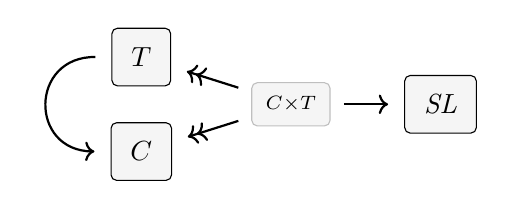
\begin{tikzpicture}
				\node[dpadded] (SL) at (-1.0,0) {$\mathit{SL}$};
				
				\node[dpadded,light pad] (CT) at (-2.9, 0){$\scriptstyle C \times T$};
				\node[dpadded] (C) at (-4.8, -0.6) {$C$};
				\node[dpadded] (T) at (-4.8, 0.6) {$T$};
				
				%				\node[dpadded, dashed,color=violet] (X) at (6.5,0) {$X$};
				%				\draw[arr, color=violet] (X) -- (S);
				%				\draw[arr, color=violet] (X) -- (C);
				%				\draw[arr, dashed, color=violet] (X) -- (SC);
				
				\draw[arr, ->>] (CT) -- (C);
				\draw[arr, ->>] (CT) -- (T);
				\draw[arr] (CT) -- (SL);
				\draw[arr] (T) to [bend right=90, looseness=2] (C);
		\end{tikzpicture}
	\end{center}
\end{constr}

\setcounter{section}{3}
\setcounter{theorem}{4}
\begthm{prop}{prop:consist}
%joe15: it's not ``in particular''.  
%$\bbr{\dg M}^* \in \bbr{\dg M}_0^*$; in particular, if $\dg M$ is consistent,
$\bbr{\dg M}^* \in \bbr{\dg M}_0^*$, so if $\dg M$ is consistent,
then $\bbr{\dg M}^* \in \SD{\dg  M}$.
\end{prop}
	
	\setcounter{section}{4}
	\setcounter{subsection}{1}
	\subsection{Factor Graphs} 
	\label{sec:factor-graphs}
	Factor graphs
%oli21: The original paper is actually really persuasive and arguably a better introduction
%	\cite{wainwright2008graphical,kschischang2001sumproduct},
	\cite{kschischang2001sumproduct},
	like PDGs, generalize BNs 
%oli21: softening:
	in some sense
	and have a low barrier to adding observations.  
	%oli21: I still would defend this, but let's not go there right now.
%	Moreover, their failure to
%	normalize in general may be viewed as a way of representing some inconsistency.
	In this section, we consider the relationship between factor graphs (FGs) and PDGs.
	
	\begin{defn}
		A \emph{factor graph} $\Phi$ is a 
		%oli21
		% collection
		set
		of random variables
		$\mathcal X = \{X_i\}$ and \emph{factors}
		$\{\phi_J\colon \V(\mat X_J) \to \mathbb R_{\geq0}\}_{J \in
			\mathcal J }$
		where each $\mat X_J \subseteq \mathcal X$.  
		more precisely, each factor $\phi_J$ is associated with a subset
		$\mat X_J\subseteq \mathcal{X}$ of variables, and maps
		joint settings of $\mat X_J$ to non-negative real numbers.
	\end{defn}
	We will refer to a factor graph $\Phi$,
	together with a vector of non-negative weights $\{ \theta_J \}_{J \in \mathcal J}$,
	as a \emph{weighted factor graph} (WFG) , which 
	specifies a distribution 
	\[ {\Pr}_{(\Phi,\theta)}(\vec x)
		= \frac{1}{Z_{\Phi,\theta}} \prod_{J \in \cal J} \phi_J(\vec
		x_J)^{\theta_J} \]
	and also a canonical scoring function 
	\begin{equation}
		\GFE_{(\Phi,\theta)}(\mu)
		:= \!\E_{\vec x\sim\mu}\left[  \sum_{J \in
			\cal J} \theta_J \log\frac1{\phi_J(\vec
			x_J)}\right] - \H(\mu)  , 
		\label{eqn:free-energy}
	\end{equation}
	which $\Pr_{(\Phi,\theta)}$ minimizes, called the \emph{variational Gibbs free energy}
	\cite{mezard2009information}. 
	Here $\vec{x}$ is a joint setting on all of the variables,
	$\vec{x}_J$ is the restriction of $\vec{x}$ to only the
	variables $X_J$, and $Z_{\Phi,\theta}$ is the constant required to
	normalize the distribution. 
	%oli21:
	An unweighted FG $\Phi$ defines a distribution $\Pr_\Phi$ and $\GFE_{\Phi}$ by implicitly taking every $\theta_J = 1$;
	the WFGs generated by other settings of $\theta$ are known as $\Phi$'s exponential family.
	
	The cpds of a PDG straightforwardly constitute the data of a factor graph. 
	
\begin{defn}[PDG to FG]\label{def:PDG2fg}
	If $\dg M = (\Gr, \mat p)$ is an unweighted PDG, define   
	the associated FG $\FGof{\dg M}$ on the 
	variables $\nvvars$ by
	%oli21: make sure we talk about J, this is ambiguous.
	% I am so sure I did this properly before at some point...
	% taking the factors to be given by the edges in $\Ed^{\dg M}$, 
	taking $\mathcal J := \Ed^{\dg M}$ to be the set of edges, %$X_{\ed LXY} := \{X,Y\}$, 
	%oli21: also changing "X" to "Z" because of possible name conflict.
	% and for an edge $L$ from $X$ to $Y$, taking
	% $X_{L} = \{X,Y\}$, and $\phi_L(x,y)$ to be $(\bp^{\dg M}(x))(y)$.
	and for an edge $L$ from $Z$ to $Y$, taking
	$X_{L} = \{Z,Y\}$, and $\phi_L(z,y)$ to be $(\bp^{\dg M}(z))(y)$.
	%oli21: 
	We extend the transformation to one that converts a (weighted)
	PDG $\dg M' = (\dg M, \beta)$ to a WFG $\WFGof{\dg M'} := (\FGof{\dg M}, \beta)$ by taking $\theta_L = \beta_L$.
\end{defn}
	Using essentially the same trick as \cref{constr:hyperedge-reducton},
	we can encode a factor graph as an assertion about the unconditional
	probability distribution over the variables associated to each
	factor.  
	
\begin{defn}[FG to PDG] \label{def:fg2PDG}
	%oli21:
	For a FG $\Phi$ over $\nvvars$, let $\PDGof{\Phi}$ be
	% For a WFG $\Psi = (\Phi,\theta)$, let $\PDGof{\Psi}$ be
	%oli21:
	% the unweighted PDG whose variables are the variables in $\Phi$ together
	the unweighted PDG consisting of
% the variables in $\Phi$ together
% with $\var 1$ and a variable $X_J := \prod_{j \in J} X_j$ for every factor $J \in \mathcal J$%
\begin{itemize}
	\item the variables in $\Phi$ together
   with $\var 1$ and a variable $X_{\!J} := \prod_{j \in J} X_j$ for every factor $J \in \mathcal J$%
   , and
   \item edges ${\var 1} \!\to\! X_{\!J}$ for each $J$ and $X_{\!J} \!\tto\! X_j$ for each $X_j \in \mat X_J$,
   \item where $ X_{\!J} \!\tto\! X_j$ are associated with the appropriate projections, and each ${\var 1} \!\to\! X_{\!J}$ is associated with the unconditional joint distribution on $X_J$
   %symols perhaps unhelpful 
   % $\bp[\var 1\to X_{\!J}]$
    obtained by normalizing $\phi_J$. %$\sum_{\mat x_{J}}\phi_J(\mat x_J) = 1$.
\end{itemize}
The process is illustrated in \cref{fig:fg2PDG}.
%oli21: was extremely tricky to read and edit in its fragle run-on-sentence form. I
% split it into the bullets above.
	% , and whose edges consist of projections $X_J \tto X_j$ for each $X_j \in X_J$ and
	% unconditional joint distributions ${\mathsf 1} \to X_J$ with
	% associated cpd $\bp[J]$ equal to the joint distribution on $X_J$ obtained by
	% normalizing $\phi_J$. 
%oli21: 
% more careful here also
% Finally, we extend the transformation to WFGs $(\Phi, \theta)$ by taking the  \valpha{$\alpha_L = $}$\beta_L := \theta_L$. ``
We extend the transformation to WFGs $\Psi=(\Phi, \theta)$ by taking $\beta_L := \theta_L$, and denote the resulting (weighted) PDG by $\PDGof{(\Phi, \theta)}$.
\valpha{Doing so leaves $\alpha_L=1$ to be compatible with our default, but we will see that setting $\alpha_L := \theta_L$ is a better translation; for this we write $\PDGof{\Phi, \theta, \theta}$, or $\PDGof{\Psi -}$ 
to avoid unpacking the WFG $\Psi$; 
more generally, we write $\PDGof{\mathcal O,\beta,\alpha}$ for the PDG formed by attaching weight vectors $\beta$ and $\alpha$ to the conversion of an unweighted object $\PDGof{\mathcal O}$.}
\end{defn}
	\begin{figure*}[htb]
		\centering
		% \begin{subfigure}{0.5\linewidth}\centering
		\scalebox{0.8}
		{
			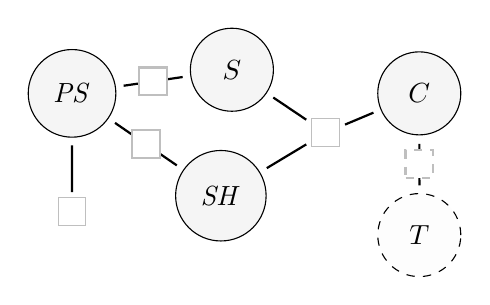
\begin{tikzpicture}[center base, xscale=1.4,
				fgnode/.append style={minimum width=3em}]
				\node[factor] (prior) at (1.65,-1) {};
				\node[factor] (center) at (3.95, 0){};
				
				\node[fgnode] (PS) at (1.65,0.5) {$\mathit{PS}$};
				\node[fgnode] (S) at (3.1, 0.8) {$S$};
				\node[fgnode] (SH) at (3.0, -0.8) {$\mathit{SH}$};
				\node[fgnode] (C) at (4.8,0.5) {$C$};
				
				\draw[thick] (prior) -- (PS);
				\draw[thick] (PS) --node[factor, fill=white](pss){} (S);
				\draw[thick] (PS) --node[factor, fill=white](pssh){} (SH);
				\draw[thick] (S) -- (center) (center) -- (SH) (C) -- (center);
				
				%					\node[dpadded, fill=blue] (1) at (2.5,-2) {1};
				%					
				%					\draw[blue!50, arr] (1) -- (prior);
				%					\draw[blue!50, arr] (1) -- (center);
				%					\draw[blue!50, arr] (1) -- (pss);
				%					\draw[blue!50, arr] (1) -- (pssh);
				
				
				\node[fgnode, fill opacity=0.02,dashed] (T) at (4.8, -1.3) {$T$};
				\draw[thick,dashed] (T) -- node[factor, fill=white]{}  (C);	
		\end{tikzpicture}}
		~\vrule~
		% \end{subfigure}
		% \begin{subfigure}{0.5\linewidth}\centering
		\scalebox{1}
		{
			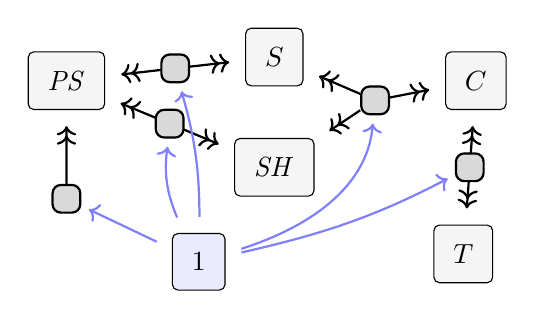
\begin{tikzpicture}[center base, xscale=1.6,
				newnode/.style={rectangle, inner sep=5pt, fill=gray!30, rounded corners=3, thick,draw}]
				\node[newnode] (prior) at (1.65,-1) {};
				\node[newnode] (center) at (4.1, 0.25){};
				
				\node[dpadded] (PS) at (1.65,0.5) {$\mathit{PS}$};
				\node[dpadded] (S) at (3.3, 0.8) {$S$};
				\node[dpadded] (SH) at (3.3, -0.6) {$\mathit{SH}$};
				\node[dpadded] (C) at (4.9,0.5) {$C$};
				
				\draw[arr, ->>, shorten <=0pt] (prior) -- (PS);
				\draw[arr, <<->>] (PS) --node[newnode](pss){} (S);
				\draw[arr, <<->>] (PS) --node[newnode](pssh){} (SH);
				\draw[arr, <<-, shorten >=0pt] (S) -- (center); 
				\draw[arr, <<-, shorten >=0pt] (SH)-- (center); 
				\draw[arr, <<-, shorten >=0pt] (C) -- (center);
				
				\node[dpadded, fill=blue] (1) at (2.7,-1.8) {1};
				
				\draw[blue!50, arr] (1) -- (prior);
				\draw[blue!50, arr] (1) to[bend right=30] (center);
				\draw[blue!50, arr] (1) to[bend right = 5] (pss);
				\draw[blue!50, arr] (1) to[bend left = 10] (pssh);
				
				
				\node[dpadded] (T) at (4.8, -1.7) {$T$};
				\draw[arr, <<->>] (T) -- node[newnode](tc){}  (C);	
				
				\draw[blue!50, arr] (1) to[bend right = 10] (tc);
		\end{tikzpicture}}
		% \end{subfigure}
		
		\caption{
			Conversion of the PDG in \cref{ex:smoking} to a factor graph
			according to \cref{def:PDG2fg} (left), and from that factor graph back
			to a PDG by \cref{def:fg2PDG} (right). 
			In the latter, for each $J$ we intorduce a new node $X_J$ (displayed as a
			smaller darker rectangle) whose values are joint settings of the
			variables connected it, and also an edge $1 \to X_J$ 
			(blue)
			%FIXME
			to which we associate with the unconditional 
			distribution given by normalizing $\phi_J$.
		} 
		\label{fig:fg2PDG}
	\end{figure*}

	PDGs are directed graphs, while factors graphs are undirected. The
	map from PDGs to factor graphs thus loses some important structure;
	as shown in
	\Cref{fig:fg2PDG},
	the transformations can change the graphical structure significantly.
%oli21: edited and aadded back an old proposition to tell story. 
% you are welcome to cut it if you don't like the story here.
\attn{
Nevertheless, the conversions
preserve enough that cycling between them does not meaningfully alter the distribution they represent.
% they 'meaningfully' is because technically
% we've introduced more variables, but marginalizing to any shared subset is
% always equivalent.
\begthm{prop}{prop:fg-pdg-lossless}
%oli21: here's an excellent example of why I dislike the notation
% of using subscripts to transform variables. Now we need a new letter for the
% factor graphs themselves, because the meaning of "{\dg M}" is ambiguous: is it the 
% model or the transformation? Addinga prime to distinguish the PDG over the
% transformation does not help, because this further 
% suggests that there's already a PDG called {\dg M}, which there is not. The
% same is true for $\Phi$; I originally used "F" but expanding to 
% $\Phi, \theta$  was a better-looking option in this case.\
% For now, I've changed M to N to prevent the syntactic clash.
	For a WFG $(\Phi,\theta)$, 
	$\Pr_{\WFGof{\PDGof{\Phi,\theta}}} \!\cong\! \Pr_{(\Phi,\theta)}$;
	\def\freshpdgsymbol{{\dg N}}
	for a PDG $\freshpdgsymbol = (\Gr, \mat p, \beta)$, we have $\Pr_{\PDGof{\WFGof{\freshpdgsymbol}}} \cong \Pr_{\freshpdgsymbol}$.
\end{prop}
%oli21: altering the focus.
% in the case where every weight is the same,
% then both conversions preserve the semantics 

Despite isomorphism between the two representations,
they not generally share semantics. But they do in the case
where every weight is the same, for the particular value of $\gamma$ equal to the shared weight}. 

\begthm{theorem}{thm:pdg-is-fg}

If $\dg M$ is a PDG such that for some $\gamma >0$, we have that $\beta_L\!
= \gamma$ for all  $L$, then
$\bbr{\dg M}_{\gamma} = \gamma\,\GFE_{ \WFGof{\dg M} }$ and
$\bbr{\dg M}_{\gamma}^* = \{\Pr_{ \WFGof{\dg M}} \}$.

\end{theorem}
\attn{
In particular, 
% the $\gamma=1$ unique-distribution semantics for an unweighted PDG
$\bbr{ - }_1^*$
simply regards an unweighted PDG as a factor graph.
\begin{coro}\label{coro:justafg}
	% If $\dg M$ is an unweighted PDG, then 
%	If $\dg M = (\Gr, \mat p)$ is an unweighted PDG, then 
	$\displaystyle\bbr{\Gr, \mat p}_1^* 
%		= \frac{1}{Z_{\dg M}}\prod_{\ed LXY \in \Ed^{\dg M}} \bp^{\dg M}(Y \mid X)
\propto \prod_{\ed LXY \mathrlap{\in \Ed^{\dg M}}} \bp(Y \mid X)$
%
\end{coro}
% Conversely, viewing a factor graph
}

\begthm{theorem}{thm:fg-is-pdg}
Given a factor graph $\Phi$, 
and a constant vector $\kappa \!=\! \{ k \}_{J \in \cal J}$ for some fixed $k$, 
%we have 
$\GFE_{\Phi, \kappa}\!= \nicefrac{1}{k}\bbr{\PDGof{\Phi,\kappa}}_{k} + C$  
for some constant $C$, so $\Pr_{\Phi, \kappa}$ is the unique element of 
$\bbr{\PDGof{\Phi,\kappa}}_{k}^*$. 
\end{theorem}
%
%\attn{
%So fixing every $\alpha_{L}\!=\!\beta_{L}\!=\!\gamma\!=\! 1$, PDGs are a restrictive interface (requiring there to be a variable $Y_J \in \mat X_J$ such that $\sum_{y
%%oli: this notation is a bit much; I introduced it but am leaving it out for now.
% 	% \in \V(Y_L)
%} \phi_{J}(y, \mat x) = 1$, for each $\phi_J$ to be a cpd) to factor graphs. 
%%	\footnote{The nature of the restriction is that each factor $\phi_J$, must normalize over the tail of the arrow.}
%}%
%oli21: rewrite paragraph continue the train of thought
% These theorems are quite restrictive:  Theorem~\ref{thm:pdg-is-fg}
% applies only to PDGs where all the uncertainties $\beta_L$ are
% identical,  while Theorem~\ref{thm:fg-is-pdg} applies only to factor
% graphs where all weights $\Theta_J$ are identical.  
% We can generalize
% Theorem~\ref{thm:pdg-is-fg} slightly to the case where the ratio of
% $\alpha_L$ to $\beta_L$ is a constant.
\Cref{thm:pdg-is-fg,thm:fg-is-pdg} are quite restrictive, as they only apply
for a specific $\gamma$, and only where the weights are identical. The first 
restriction is fundamental, but the second can be eliminated
\valpha{by allowing $\alpha_L$ to vary together with $\beta$, as in our second translation.

\begthm{theorem}{thm:pdg-is-fg2}
If $\dg M$ is a PDG such that for some $\gamma >0$, we have that
$\beta_L = \valpha{\alpha_L} \gamma$ for all  $L$, then
$\bbr{\dg M}_{\gamma} = \gamma\,\GFE_{\WFGof{\dg M}} $ and
$\bbr{\dg M}_{\gamma}^* = \{\Pr_{\WFGof{\dg M}} \}$.
\end{theorem}


\begthm{theorem}{thm:fg-is-pdg2}
For every factor graph $\Phi$, and EVERY vector $\theta$ over $\cal J$ 
we have that
$\GFE_{(\Phi,\theta)} \!=\! \nicefrac1{\gamma} \bbr{\PDGof{\Phi,\theta, \nicefrac\theta\gamma}}_{\gamma} + C$  
for some constant $C$, so
$\Pr_{(\Phi, \theta)}$ is the unique element of $\bbr{\PDGof{\Phi,\theta, \nicefrac\theta\gamma}}_{\gamma}^*$. 
\end{theorem}
\begin{coro}
	For all WFGs $\Psi$, $\bbr{\PDGof{\Psi-}}^*_1 = \{ \Pr_{\Psi} \}$; 
	similarly,
	$ \bbr{\Gr, \mat p, \beta, \beta} \propto \prod_L \bp^{\beta_L}$.
\end{coro}
This strengthens \cref{coro:justafg}: by fixing $\alpha_L = \beta_L$, the $\gamma=1$ semantics captures the behavior of the entire exponential family of $\dg M$, as viewed as a set of factors.
%correctly scores the entire exponential family of $\PDGof{\Phi}$
}

The key step in proving \Cref{thm:fg-is-pdg,thm:pdg-is-fg}
(and in the proofs of a number of other results) involves 
rewriting  
$\bbr{\dg M}_\gamma$ as follows: 
\begin{prop}[restate=prop:nice-score,label=prop:nice-score]% \label{}
Letting $x^{\mat w}$ and $y^{\mat w}$ denote the values of
$X$ and $Y$, respectively, in $\mat w \in \V(\dg M)$, 
we have 
\begin{equation}\label{eq:semantics-breakdown}
\begin{split}
\bbr{\dg M}(\mu) =  \!\!\!\sum_{\mat w \in \V(\dg M)} \!\!\! \mu(\mat w) \Bigg\{
\sum_{ X \xrightarrow{\!\!L} Y  }
\bigg[\,
\color{gray}\overbrace{\color{black}
\!\beta_L \log \frac{1}{\bp(y^{\mat w} |x^{\mat w})}
}^{\color{gray}\smash{\mathclap{\text{log likelihood / cross entropy}}}} + \\[-0.5em]
\color{gray}\underbrace{\color{black} 
(\valpha{\alpha_L}\gamma - \beta_L ) \log \frac{1}{\mu(y^{\mat w} |x^{\mat w})} 
}_{\color{gray}\smash{\mathclap{\text{local regularization (if $\beta_L > \gamma$)}}}}\bigg] - \underbrace{\color{black}
\gamma \log \frac{1}{\mu(\mat w)}
}_{\color{gray}\smash{\mathclap{\text{global
			regularization}}}}\color{black} \Bigg\} .
\end{split}
\end{equation}
\end{prop}

For a fixed $\gamma$, the first and last terms
of \eqref{eq:semantics-breakdown} are equal to a scaled
version of the free energy, $\gamma\GFE_\Phi$, for $\phi_J = \bp$ and $\theta_J
= \nicefrac{\beta_L}{\gamma}$.  
If, in addition, $\beta_L = \valpha{\alpha_L}\gamma$ for all
$L$, then
the local regularization term disappears, giving us
the desired correspondence. 

Although both $\theta$ and $\beta$ are measures of confidence, 
the way that a factor graph varies with $\theta$ 
is quite different from the way a PDG
varies with $\beta$. Increasing $\theta_L$ results in higher mass on the most likely worlds (even if such worlds already had more mass than $\bp$ would suggest), while increasing $\beta_L$ results in a distribution that is closer to marginalizing to $\bp$. 
\commentout{
	We now explain how the middle term may be viewed as a ``local'' regularization,
	and why including such a term is necessary for the semantics to 
	view our cpds $\mat p$ as assertions about probability
}

%joe18*: reinstating some material from before, with slight rewriting.
\Cref{eq:semantics-breakdown} also makes it clear that 
%oli21:
fixing $\gamma$ and
taking $\beta_L = \valpha{\alpha_L} \gamma$ for all edges $L$ is
essentially necessary to get \Cref{thm:pdg-is-fg,thm:fg-is-pdg}.
%oli21*: this is the oposite of what we wanted to say.
%. The equality HOLDING is what gives us strange behavior.  Rewriting.
%	If this equality does not hold, then we can get some 
Of course, fixed $\gamma$ precludes taking $\lim_{\gamma\to0}$, so \cref{prop:consist} does apply. 
This is reflected in some strange
behavior in factor graphs trying to capture the same phenomena as
PDGs, as the following example shows.

\begin{example}\label{ex:overdet}
Consider the PDG $\dg M$ containing just $X$ and $1$, and two edges
$p, q: 1 \to X$.
%joe8:
(Recall that such a PDG can arise if we get different information about the
probability of $X$ from two different 
sources; this is a situation we
certainly want to be able to capture!)
Consider the simplest situation, where $p$ and $q$ are both associated
with the same distribution on $X$%
; further suppose that the agent is certain about the distribution, so
$\beta_p = \beta_q = 1$.
For definiteness, suppose that
$\V(X) = \{x_1,x_2\}$, and
that the distribution associated with both edges is $\mu_{.7}$, which ascribes
probability $.7$ to $x_1$. Then, as we would hope  $\bbr{\dg M}^* =
\{\mu_{.7}\}$; after all, both sources agree on the information.
However, it can be shown that 
$\Pr_{\WFGof{\dg M}} = \mu_{.85}$, so  $\bbr{\dg M}_1^* = \{\mu_{.85}\}$.
\end{example}


%The scoring function that we use for PDGs can be viewed as
%extending ${\GFE}_{\Phi,\theta}$ by including
%the local regularization term.
%As $\gamma$ approaches zero,
%the importance of the global regularization terms decreases relative
%to that of the local regularization term.

\valpha{
The behavior in \cref{ex:overdet} also sheds some light on the nature of $\alpha$.
Because a factor graph fuses $\alpha_L = \beta_L$, duplicating an edge $L$ effectively doubles both (it doubles $\theta_L$). If one believes that $p$ and $q$ describe independent actions on $X$, then effectively doubling $\alpha_p$ may be appropriate, but this is not acceptable if we want to merely record probabilistic observations. The desired behavior can be captured with a PDG in several ways, all of which are inaccessible to factor graphs: we can increase the reliability $\beta$ for one of the edges (fixing $\alpha$), add purely observational edges that have $\alpha_L=0$, or ignore the qualitative half by taking the limit as $\gamma \to 0$.
}


\subsection{Dependency Networks}

PDGs are closely related to Dependency Networks, or DNs
\cite{heckerman2000dependency}. The data of a DN is also an unstructured
collection of cpds, but the cpds are attached to nodes rather than edges, so
there must be exactly one per node.  \citeauthor{heckerman2000dependency} also
emphasize the benefit of being able to supply arbitrary data in the cpds,
without enforcing the consistency constraints.


\begin{defn}
A Dependency Network is a tuple $\mathcal D = (\Gr, \mat p) $, where $\Gr = (\nvvars,\Ed)$ is a
directed graph of variables, and $\mathcal P$, gives for each $X \in \N$ a positive%
	\footnote{that is, each cpd $\bp[X]$ has no zero entries}
cpd $\bp[X](X \mid \Pa^{\Gr}(X))$, where $\Pa^{\Gr}(X)$ are the parents of $X$ in $\Gr$.
Together with a total order $\prec$ on $\N$,
$\mathcal D$ defines a joint distribution $\Pr^\prec_{\mathcal D}$ on $\V(\N)$ via an \emph{ordered Gibbs sampler}. Concretely, for $t= 1,2, \ldots$, the process of going through though the variables in order, and re-sampling
\[
	 X_i^{(t)} \sim \bp[i]\left(X_i ~\big|~ x_1^{(t)}, \ldots, x_{i-1}^{(t)}, x_{i+1}^{(t-1)}, \ldots, x^{(t-1)}_{n} \right) 
%		= \bp[i](X_i \mid \mat{pa}^{\Gr}(i)) 
\]
results in a Markov chain of joint variable settings
\[ \mat X^{(1)} \to \mat X^{(2)} \to \ldots \to \mat X^{(t)} \to \ldots \]
that, %so long as each $\bp[X]$ is positive,%
limits to a unique stationary distribution, which we take to be the definition of $\Pr^\prec_{\mathcal D}$.
\end{defn}

The dependence on the order is artificial in the case that the DN is ``consistent'', which in the authors parlance implies that it also has their favored independencies.\footnote{Interestingly, any BN $\mathcal B$ is an ``inconsistent'' dependency network, despite the fact that the Gibbs sampler whose order $\prec$ is a topological sort  of $\cal B$, generates $\Pr_{\mathcal B}$.}

\begthm[\citeauthor{heckerman2000dependency}]{theorem}{thm:dns-uniq}
%Theorem 1. (wrapped into definiton above)
%An ordered Gibbs sampler applied to a dependency network for $\mat X$, where each $X_i$ is discrete and each local distribution $\bp[X](x \mid \mat{pa}(X))$ is positive, has a unique stationary joint distribution for $\mat X$.  
If a dependency network $\mathcal D \!=\! (\Gr, \mat p)$ over variables $\N$ is consistent with a positive joint distribution $p$,
in that $p(X \mid \N\setminus \{X\}) = \bp[X](X \mid \Pa^{\Gr}(X))$ for all $X \in \N$,
 then $\Pr_{\mathcal D}^\prec = p$.
\end{theorem}

A dependency network $\mathcal D$, together with any a vector of confidences $\beta$ for the cpds on each variable
% (defaulting to $\beta_X=1$) 
can be naturally regarded as a PDG $\PDGof{\mathcal D, \beta}$ 
via the same translation used for a Bayesian Network.
Although on the surface PDG and DN semantics are quite
different,
the former subsumes the latter, as the next results show.


%\begin{lemma}
%	A distribution $\mu$ that locally minimizes $\IDef{\PDGof{\mathcal D, \beta}}$ satisfies all of the independencies of $\mathcal D$.
%\end{lemma}


\begthm{conj}{thm:dns-are-pdgs}
%oli21: updating theorem statement
% If $\mathcal D = (\N, \Ed, \V, \mathcal P)$ is a consistent dependency network with a positive stationary distribution $p^*$ of its sampling procedure, then the PDG $\PDGof{\mathcal D} = (\N, \mathit{merge}(\Ed), \V, $$\mathcal P, \mat 1\valpha{, $\mat 1$})$, then $\bbr{\PDGof{\mathcal D}} = p^*$.
If $\mathcal D$ is a consistent dependency network,
%with positive local distributions,
then for all positive vectors $\beta$, and all orders $\prec$, we have that
%$\SD{\PDGof{\mathcal D, \beta}} =  \{ \Pr_{\cal D}^\prec \}$.
$\bbr{\PDGof{\mathcal D, \beta}}^* =  \Pr_{\cal D}^\prec$.
%, where $\Pr_{\cal D}^\prec$ is the unique stationary distribution of the $\prec$-ordered Gibbs sampling procedure. 
\end{conj}

Inconsistent DNs still define a unique distribution, but we cannot hope that it 
will be the same one as generated by the PDG, owing to the fact that
the Gibbs sampler defined by \citeauthor{heckerman2000dependency} is dependent
on the (arbitrary) fixed order used in sampling.
A PDG can simulate the effect of the order with the reliability $\beta$.

\begin{conj}
If $\mathcal D$ is a dependency network over the variables
$X_1 \prec X_2  \ldots  \prec X_n$ is a total order on the variables, and $\beta$ is a vector over the edges
%oli21: to preemptively eliminate some confusion:
% (which have a 1-1 correspondence with variables in a DN) 
such that  $\beta_1 \ll\beta_2 \ll \ldots \ll \beta_n$, 
then $\Pr_{\cal D}^{\prec} = \bbr{\dg M; \beta}^*$
\end{conj}

A \emph{random scan} Gibbs sampler, rather than cycling though variables in a 
particular order, draws the next variable index to update randomly.
Given a distribution $d$ over $\N$,
let $\mathit{RScan}(d)$ be the random scan Gibbs sampling procedure that draws
the next variable to update from $d$. $\mathit{RScan}(d)$ also has a unique stationary distribution, $\Pr_{\mathcal D}^d$, which is equal to $\Pr_{\cal D}^{\prec}$ for any $d$ and $\prec$ if $\mathcal D$ is a consistent DN. This more symmetric procedure is captured nicely by PDG semantics.

\begin{conj}\label{thm:dns-are-completely-pdgs}
	Let $d(X) \propto \beta_X$. Then
	$\Pr_{\mathcal D}^d = \bbr{\PDGof{\mathcal D, \beta}}^*$, whether or not $\mathcal D$ is consistent.
\end{conj}

%\Cref{thm:dns-are-completely-pdgs} provides a the question left open by \citeauthor{heckerman2000dependency} 

%\appendix
%\clearpage
%\onecolumn
%\section{Proofs}
%\begin{lemma}
%	content
%\end{lemma}
%
%\recall{thm:dns-are-pdgs}
%\begin{proof}
%	%	We start by showing that 
%	Let $\dg D := \PDGof{\mathcal D, \beta}$ be the PDG corresponding to  $\mathcal D$,
%	$S := \SD{\dg D}$ be the set of distributions that match the local probabilities of $\mathcal D$,%
%	\footnote{Technically, because of the hyper-graph conversions, these are actually distributions that include joint variables, but for the same reasons as in the BN case, the joint variables and their projections can safely be ignored.}
%	and $q := \bbr{\dg D}^*$ be the unique distribution picked out by PDG semantics; by \cref{prop:}, we know that $q \in S$.
%	As $\cal D$ is a consistent DN, there is a positive $p$ such that $p \in S$ and $p(X \mid \Pa(X)) = p(X \mid \N \setminus \{X\})$ for each $X$. 
%	In search of a contradiction, suppose that $p \neq q$. Since $q$ uniquely minimizes $\bbr{\dg D}$, and $\Inc_{\dg D}(p) = \Inc_{\dg D}(q) = 0$, we must have $\IDef{\dg D}(q) < \IDef{\dg D}(p)$. 
%	
%	\begin{align*}
%		%
%	\end{align*}
%\end{proof}
%
%
\bibliography{joe,z,allrefs}
\end{document}
